Given the size of the tree to be explored (at least 400 million nodes), a root parallelisation strategy on computers could not be applied. A 11 million nodes tree require about 2 Go of RAM. Should it be timed by 40 and the number of core, there would be not enough RAM.
\bigskip
\begin{center}
	\begin{tabular}{ | c | c | c |}
		\hline  & Before & After \\ \hline
		\hline  
		Percentage of memory used & 39\% & 93\% \\
		\hline  
		Total physical memory & 3981 MB & 3981 MB \\
		\hline  
		Free physical memory & 2411 MB & 255 MB \\
		\hline
	\end{tabular}
	
	Comparison between the RAM available before and after\\the creation of a tree (and its buffer) composed by 10 940 207 nodes.
\end{center}
\bigskip

With this in mind, a tree parallelisation strategy has to be implemented on the computer. In this method, multiple threads share the same tree, the exploration is done the same way as it is with one thread.
\begin{figure}[H]
\centerline{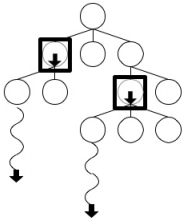
\includegraphics[]{Parallelisation/Computer/Img/Tree.png}}
\caption{\label{fig:TreeParallelization}\textit{Tree parallelization}}
\end{figure}
\begin{figure}[H]
\centerline{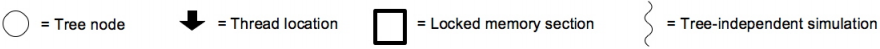
\includegraphics[width=0.7\textwidth]{Parallelisation/Computer/Img/legend.png}}
\end{figure}
The main problem of this method is that multiple threads can access the same node and corrupt data given by another thread. To avoid such problems, we will be using \textit{virtual loss} and \textit{local mutexes}.

Should a thread go through a node, it automaticaly increases the value of its visit counter. This will virtually decrease the winning rate of the node and therefore decrease its attractiveness.

Each node also has a boolean to serve as a lock in order to prevent concurency. Its access is done in a critical section (atomic capture). Should a thread access a locked node, it will stop exploring and start its simulations.

This method of parallelization can be done by multithreading the \textit{While // loop simulations} descriped in the base algorithm implementation\ref{fig:MCTSAlgorithmOMP}. Using OpenMP, this is easily implented with a single \#pragma statement :\\
\textbf{\#pragma omp parallel shared(i,timeend)}\\
where \textit{i}, the number of simulation run and \textit{timeend}, the time until simulations are to be run are defined as shared variables.

In order to prevent any conflict between threads, a small critical section has to control the lock of the nodes. Placing the following statement before \textit{node->getLock()} do the job :\\
\textbf{\#pragma omp critical}

\begin{figure}[H]
\centerline{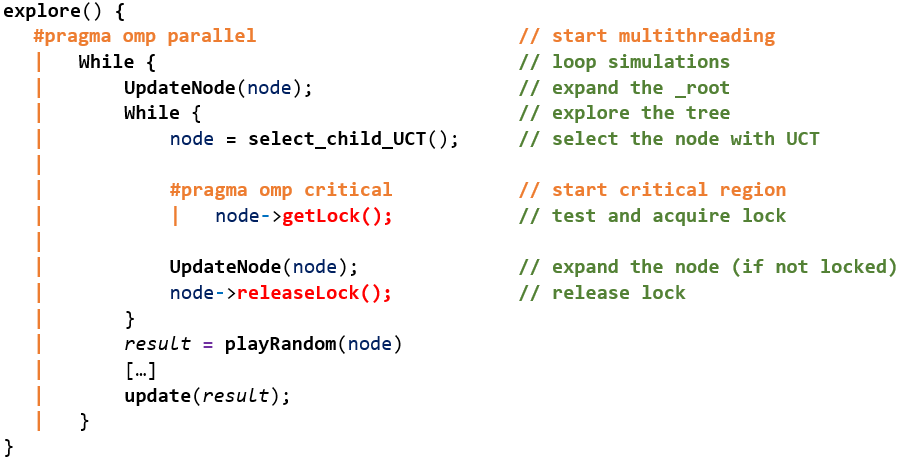
\includegraphics[width=0.7\textwidth]{Parallelisation/Computer/Img/omp.png}}
\caption{\label{fig:MCTSAlgorithmOMP}\textit{Overview of the implementation of the tree parallelization using OpenMP}}
\end{figure}
